\documentclass[12pt]{article}
\usepackage[a4paper, total={6.5in, 10in}]{geometry}
\usepackage{FunctionPlot}
\usepackage{MainTeX}
\usepackage{enumerate}
\usepackage{multicol}
\usepackage{booktabs}


\title{魔方与群}
\author{Eureka}
\date{\today}
\begin{document}
\maketitle

\section{历史进程}
魔方的基本知识

\begin{itemize}
    \item 1978年12月{\itshape Singmaster notation}(辛马斯)发明魔方的转动符号系统。
    \item 初始状态:每一个面均为同色; 可还原状态:有限次操作可复原({\bf 拧角块})
    \item 旋转的方向问题:对着相应的面按照顺时针进行旋转
    \item 魔方的影响因素:{\bf 朝向}和{\bf 位置}
\end{itemize}

\begin{figure}[!htb]
    \centering
    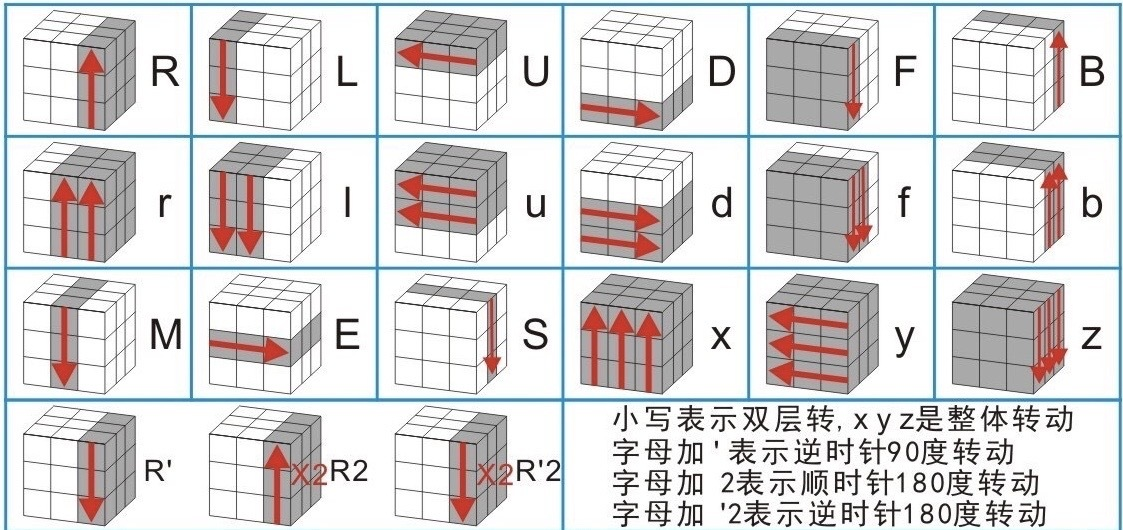
\includegraphics[scale=.35]{./rotate.jpg}
    \caption{转动符号系统说明}
    \label{转动符号系统说明}
\end{figure}



\section{几个问题}
\begin{enumerate}[(1)]
    \item 魔方处于什么状态可以被还原 ?
    \item 魔方有多少种状态 ?
    \item {\bf 怎么定义魔方的数学结构} ? \lr 这样的数学结构有什么性质 ?
\end{enumerate}


实际上魔方的{\bf 可还原状态}大概有 $8!\times 12!\times 2^{10}\times 3^7 \approx 4.3\times 10^{19}$,
但是如果我们从不严谨的角度来看待这个问题,我们可以从如下的角度思考:
魔方的种类数计算公式, 12个棱块,8个角块;每个棱块2个朝向,每一个角块3个朝向;
同时有一个限制 \lr 个棱块,角块是无法单独翻转[6]的,于是计算公式如下
\begin{align}
     N = \frac{8!\times 12!\times 2^{12}\times 3^8}{12} = 43252003274489856000
\end{align}

\begin{formal}{blue}
    1. 如果不考虑朝向,只考虑色块的位置,那么我们拧魔方的操作实际上是全体色块位置的一个 {\bf 偶置换[2]}

    \noindent2. 色块的朝向就是一个2(3)阶的循环群 $G_e = <g>, G_v = <g'>$
\end{formal}

\subsection{定理与定义}
\begin{framed}
{\bf (魔方第一基本定理)}\kaishu 
一个魔方的状态由以下的条件唯一确定:
\begin{multicols}{2}
    \begin{itemize}
        \item 每一个棱块的位置
        \item 每一个棱块的朝向
        \item 每一个角块的位置
        \item 每一个角块的朝向
    \end{itemize}
\end{multicols}

看起来似乎就是一句废话 $\sim\sim\sim$
\end{framed}

下面就是一些规定:每一个棱色块的正方向为:
魔方处于初始状态时这个位置棱块的正面色(自己选取,一般使用还原魔方的自然定义)的朝向.

下面我们为了方便,我们对魔方的全体棱块与角块进行排序(随意排序均可),从而确定每一个色块的方向是
$G_{e}^{12}$(全体12个棱块的朝向的所有情况)或 $G_v^{8}$的几个分量。

\subsection{群定义}
首先定义{\bf 魔方群} $G$,其中的乘法 $x\circ y$定义为: 先进行 $x$ 操作,然后再进行 $y$ 操作,
我们称这个群 $G$ 为魔方群(Rubik's Group).
\begin{align}
    G = \langle R, L, F, B, U, D\rangle
\end{align}


定义群 $H$ 为将魔方从初始状态变换到任意状态(包括可还原和不可还原)的全体,
其中的乘法 $x\circ y$定义为: 先进行 $x$ 操作,然后再进行 $y$ 操作.

令 $S_E(=S_{12})$ 表示棱块的位置变换全体, $S_v(=S_8)$表示角块的位置变换全体,
其中的乘法 $x\circ y$定义为: 先进行 $x$ 操作,然后再进行 $y$ 操作.

为了把(操作) $g\in H$ 对色块的作用{\bf 提取}出来,于是我们建立以下的两个群同态.
\begin{align}
    \sigma: H \lr S_E
    \hspace*{4em}
    \rho: H \lr S_v   
\end{align}

$\sigma$ 将魔方的变换 $g\in H$ 映射到这个变换对全体{\bf 棱块}的位置变换,而
$\rho$ 将对魔方的全体变换 $g\in H$ 映射到这个变换对全体{\bf 角块}的位置变换.

\begin{formal}{blue}
    比如我做一个 $R$,本质上对于 $S_E$ 来说就是一个四轮换。
\end{formal}


定义两个映射 
\begin{align}
    \begin{aligned}
        w: H & \lr G_e^{12} \\
        g & \sr w(g) 
    \end{aligned}
    \hspace*{4em}
    \begin{aligned}
        z: H & \lr G_v^{8} \\
        g & \sr z(g) 
    \end{aligned}
\end{align}

其中 $w(g)$ 的第 $i$ 个分量表示初始状态下的第 $i$ 个棱块在经过变换 $g$ 后改变的方向,
也可以认为就是初始状态下位于第 $i$ 个位置的棱块经过变换 $g$ 后改变的方向。比如

\begin{center}
    \begin{tabular}{p{.45\linewidth}p{.45\linewidth}}
        \toprule
        $g$ & $w(g)$\\
        $F$ & $\{1,0,0,0,0,1,0,0,0,0,0\}$\\
        \bottomrule
    \end{tabular}
\end{center}

实际上这个就和群的外半直积比较相似了,可以用这个方向的思路来处理:
如果有两个群 $N$ 和 $H$,以及群同态 $\psi:H \lr Aut(N)$, 则定义 $N$ 与 $H$
的外半直积 $N\rtimes H$ 成为一个群。

但是在这里我们采用的是 {\bf 降群法}(Schreire-Sims-Minktwits)来处理的。














\end{document}